\chapter{Optimized Deceleration}

Over the past two decades, Stark deceleration has enabled groundbreaking collisional~\cite{Sawyer2011,Kirste2012,Gao2018} and spectroscopic~\cite{Veldhoven2004,Hudson2006,Lev2006,Fast2018} studies of a variety of species~\cite{VanDeMeerakker2012}. 
Subsequent trap-loading greatly enhances interrogation time for such studies~\cite{Sawyer2008} and opens the door for further cooling and manipulation~\cite{Stuhl2012evap, Reens2017}. 
Zeeman deceleration has developed in parallel and enabled similar achievements for paramagnetic species. 


\section{Decelerator Geometry}

Much like related work in charged particle accelerators, a neutral particle decelerator is required to satisfy two key principles:
\begin{enumerate}
\item A particular candidate particle known as the synchronous molecule must be manipulated as desired by the device, e.g. slowed from $800-50$~m/s.
\item Other particles of similar initial conditions to the synchronous molecule must also possess similar final conditions.
\end{enumerate}
This second principle is known as phase stability, and is crucial to the overall performance of the device as far as flux or brightness is concerned.

Neutral particle decelerators face an incredible setback relative to charged particle accelerators, in that it is vastly harder to apply forces on them.
Specifically, the device I will soon describe can accelerate hydroxyl radicals at $\sim 200$~km/s/s. 
If hydroxyl cations were instead placed in the largest electric fields generated by the device of about $100$~kV/cm, they would experience an acceleration given by:
\begin{equation}
\frac{q_e\cdot E_\text{max} }{m_\text{OH}} = 5.5\times 10^9\text{ km/s/s}.
\end{equation}
This constitutes a factor of over ten million. 
But is this truly fundamental, or technically limited? 

Applying forces on neutral particles requires the application of gradients in electric field magnitude, and the magnitude of these gradients depends on the miniaturization of the geometry the electrodes.
It becomes challenging to develop a truly fair comparison, but underneath all of the details about electrodes and geometries, electric fields are always generated by charged particles, regardless of whether they are conduction band electrodes in some material.
The force on a neutral particle by a charged one scales as $r^4$, while that between charged ones scales as $r^2$.

In any case, once the factor of ten million setback is taken into account, neutrals have the nice property that only the magnitude of the field influences them, and not the direction. 
This makes it possible to generate large magnitude electric fields with the direction of the field orthogonal to the beamline, which is precisely the trick utilized in the first Stark decelerators~\cite{Bethlem1999}.
The design of this decelerator was replicated here in the Ye group, first at a length suitable for expansion with Xenon, then later with Krypton, and most recently with Neon.
Pairs of cylindrical pins are arranged alongside the beamline, so as to apply a large but localized field magnitude across it for maximum field magnitude gradient.
Successive pairs are rotated ninety degrees relative to one another, which is relevant to transverse confinement, and every fourth pin is connected up to the same backbone electrode.

\begin{figure}[ht!]
\centering
\label{decelcartoon}
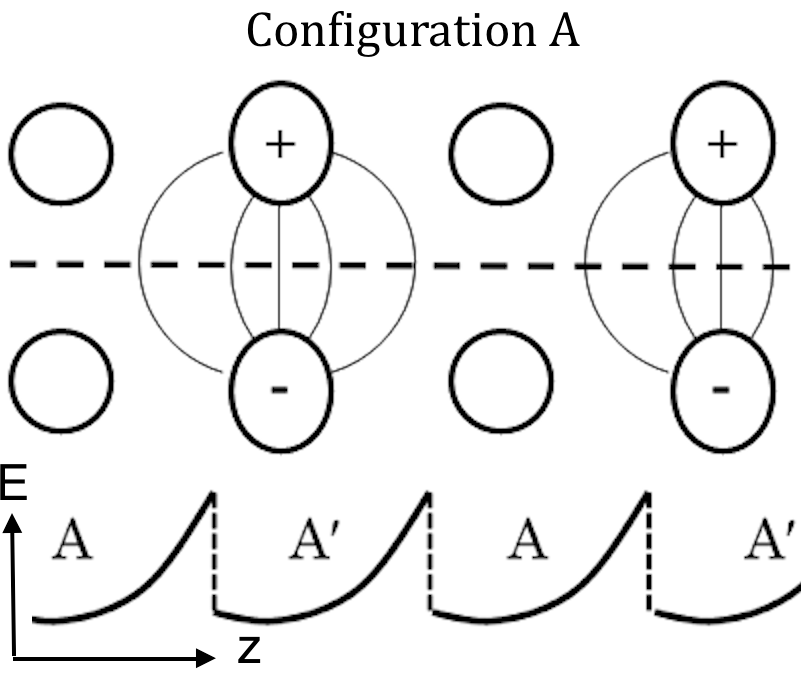
\includegraphics[width=8cm]{Slowing/chargecartoon.png}%
\caption{
Voltages, electric fields, and on-axis potential energy in a conventional pin decelerator~\cite{Bethlem1999}. Pin rotation indicated by representation as slight ellipses rather than circles. Electric fields density corresponds to the potential experienced by molecules. The horizontal dashed line indicates the central axis of the device, and the potential energy of the target or synchronous molecule as it transits this axis is shown below the pin pairs. A' indicates the translation (and rotation) of the drawn configuration of fields and voltages to the next pin pair(s). 
}
\end{figure}

Diagrams such as that shown in Fig.~\ref{decelcartoon} are useful in understanding the operation of the device.
Molecules approach a region of strong electric field, exchanging kinetic energy for internal potential energy in the case of those whose quantum state features a positive Stark shift, the only ones capable of being manipulated by such a device.
At some point, the strong electric fields are turned off, and a different region of strong electric field is turned on further along the beamline.
If the strong fields are turned off before the synchronous molecule reaches the strongest fields, i.e. partway up the hill, phase stability is obtained, because a molecule that is ahead of the synchronous one will therefore exchange a greater quantity of kinetic energy for potential energy by climbing farther up the hill before the turn-off event.
This molecule thus experiences a force restoring it to the location of the synchronous molecule.
Of course if a molecule is too far ahead, it may pass all the way through the region of highest field prior to the turn-off event. Such a molecule is no longer phase stable and will travel farther and farther from the synchronous molecule.
Thus there is a tradeoff between the deceleration capability of the device and the volume of its phase stable region.

\begin{figure}[t!]
\centering
\label{variousphaseangles}
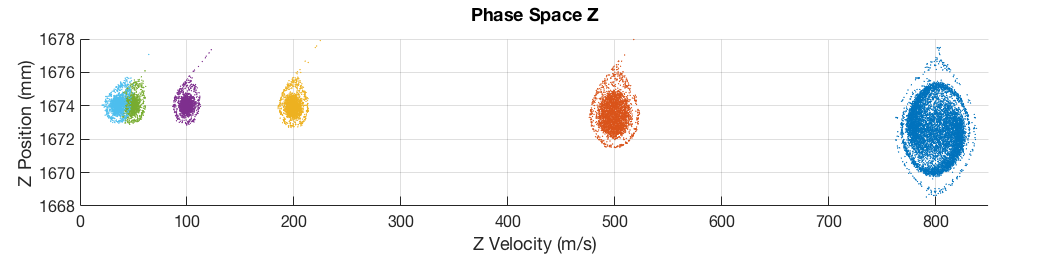
\includegraphics[width=\linewidth]{Slowing/phaseangles.png}%
\caption{
Longitudinal phase space plots of a Stark decelerator with varying final velocity. From left to right, $v_f=33, 50, 100, 200, 500, 800$~m/s. Note how the size of the populated area reduces as the final speed is reduced.  This is a direct reflection of how closely the synchronous molecule approaches the charged pin-pair, which in turn controls how far ahead a nonsynchronous molecule may be while still experiencing a restoring force. Note also how the size reduces much more significantly between $800-500-200$~m/s then for any of the other speed reductions. This is described further in the main text. 
}
\end{figure}

This can be seen more directly from simulations of its behavior, such as in Fig.~\ref{variousphaseangles}. The area of the region populated by molecules reduces as the deceleration is increased.
However, the change in area seems to plateau and then stop, somewhere between $200-500$~m/s since all velocities below $200$~m/s show nearly the same area.
This can be attributed to the fact that all of these low speeds require nearly the same energy to be removed per stage of the decelerator, since the total energy removed can be calculated by the potential energy difference:
\begin{equation}
\Delta\text{PE}=\frac{1}{2}m_\text{OH}\left(v_i^2-v_f^2\right).
\end{equation}
Once $v_f << v_i$, $\Delta\text{PE}$ no longer various strongly with $v_f$:
\begin{equation}
\label{slowphasevary}
\Delta\text{PE}\sim\frac{1}{2}m_\text{OH}v_i^2\left(1-\left(\frac{v_f}{v_i}\right)^2\right).
\end{equation}

An important corollary of this idea relates to the parameterization typically used for specifying decelerator operation.
Since the devices are periodic, it is convenient to parametrize the longitudinal coordinate with an angle, called the phase angle, and chosen to vary by $180^\circ$ between one pin-pair in the next, so that a single voltage configuration applied to the backbone repeats itself after $360^\circ$.
This parametrization also allows us to work independently from the choice of pin size and pin spacings for a given device.
A decelerator is often operated so that a synchronous molecule with a given speed would always experience a turn-off event at the same phase angle $\phi$, which then allows the operation of the device to be specified by only that angle.
It follows from Eq.~\ref{slowphasevary} however that very slight changes in $\phi$ can lead to dramatic changes in the final velocity of the synchronous molecule.
In earlier iterations of the code used for programming the switching sequence of our decelerators, it was necessary to specify the phase angle down to the thousandth of a degree in order to get the desired final speed within a few meters per second, which in turn required carefully hand-exploring the function mapping phase angles to final speeds.
This is discussed further in an appendix.

It is also worth discussing some other features of the longitudinal phase space plots shown in Fig.~\ref{slowphasevary}. 
Almost all final speeds show a bullseye type pattern, with a halo of outer particles surrounding an inner core.
This is discussed extensively in~\cite{VanDeMeerakker2006}, and relates to a discussion of inefficiencies in the device that will be continued in the next section.
However, there is additional structure evident within the inner core, especially for the molecular packet with $800$~m/s final velocity.
These molecules have not had their speed modified significantly by the simulated device, in which case the activity of the device is better described as ``bunching'' the molecules than ``slowing'' them.
In the experiment, these bunched molecules would travel together with a large population of unaddressed molecules with initial longitudinal velocity and position unsynchronized with the timing of the device.
These unaddressed molecules are nonetheless transversely focused, and in some cases with better efficiency than target molecules, and so constitute a rather large background signal relative to the molecules of interest.
The reason these unaddressed molecules are not evident in this simulation is that the simulation only initializes molecules that are likely to be addressed, for reasons of runtime.
This in turn relates to the substructure evident in the inner core of the bunched molecules in Fig.~\ref{slowphasevary}.
This substructure is an artifact of incomplete phase space filling in the simulation, i.e. if the right molecules had been included in the initialization, the inner core would be uniformly filled out and not feature any swirling.
It is useful to keep an eye out for such artifacts as a way of monitoring whether the initialization assumptions of a simulation is valid. 
This swirling is not necessarily only an artifact however, and can in fact be relevant in the experiment as well.
In~\cite{Parazzoli2009}, the rotating nature of the inner core in phase space is intentionally understood and exploited for minimizing the velocity spread of a beam exiting a decelerator.

\section{Alternative Charging Configurations}

Alongside the history of achievements enabled by Stark deceleration runs a parallel ongoing saga surrounding their efficient operation. 
Many important steps have been made, not only in understanding the flaws of the canonical pulsed decelerator~\cite{VanDeMeerakker2006,Sawyer2008a}, but also in addressing them through the use of overtones~\cite{VanDeMeerakker2005a,Scharfenberg2009}, undertones~\cite{Zhang2016}, or even mixed phase angles~\cite{Parazzoli2009,Hou2013}. 
Even with these advances, the outstanding inefficiencies of the pulsed decelerator, particularly with regard to transverse phase stability, have motivated alternative geometries such as interspersed quadrupole focusing~\cite{Sawyer2008a} and traveling wave deceleration~\cite{Osterwalder2010,VandenBerg2014,Fabrikant2014}. 
Although traveling wave deceleration takes a strong step in the right direction toward truly efficient operation, it comes with costs in system complexity and high voltage engineering. 
These costs can be partially addressed by the use of combination pulsed and traveling wave devices~\cite{Quintero-Perez2013}, or even using traveling wave geometry with pulsed electronics~\cite{Hou2016,Shyur2017}. 
Others continue to pursue brand new geometries aiming to enhance transverse acceptance without abandoning more reliable pulsed electronics~\cite{Wang2016}. 

\section{Trap Oscillations}

\section{HV Isolation Strategies}

\section{Manufacturing Considerations}